\documentclass[t]{beamer}
\setlength{\parskip}{5pt}
%\usetheme{Madrid}  

\usepackage[UKenglish]{babel}
\usepackage[UKenglish]{isodate}
\cleanlookdateon

\usepackage{listings}
\usepackage{tikz}

\newtheorem{remark}{Remark}

\def\le{\leqslant}
\def\ge{\geqslant}

\def\Z{\mathbb{Z}}
\def\N{\mathbb{N}}
\def\R{\mathbb{R}}
\def\C{\mathbb{C}}
\def\Q{\mathbb{Q}}

\title{CS3230 Tutorial 3}
\author{Deng Tianle (T15)}
\date{5 September 2025}

\begin{document}

\frame{\titlepage} 

\begin{frame}{Agenda}
  Correctness proofs:
  \begin{itemize}
    \item iterative algorithm: insertion sort (Q1)
    \item recursive algorithm: `stooge' sort (Q2)
  \end{itemize}
  Divide and conquer:
  \begin{itemize}
    \item peak-finding problem (Q3-5; also LeetCode problem)
  \end{itemize}
\end{frame}
\begin{frame}[fragile]{Q1}
  Insertion sort for array $A[0\dots N-1]$:
  \begin{lstlisting}[language=C]
    for (i=1; i<N; i++) {
      x = A[i];
      for (j=i-1; j>=0 && A[j]>x; j--) {
        A[j+1]=A[j];
      }
      A[j+1]=x;
    }
  \end{lstlisting}
  Idea: for $i$ from $1$ to $n-1$, at each step make $A[0 \dots i]$ sorted by inserting $A[i]$ at the correct place (refresher: why is this sort stable?). 
  \par Q1: what does each iteration of the outer loop accomplish? Can you prove that it is so? 
\end{frame}
\begin{frame}{Q1}
  Let $B$ denote (a copy of) the original array. Loop invariant: $A[0 \dots i]$ is the sorted version of $B[0 \dots i]$ and $A[i+1 \dots N-1] = B[i+1 \dots N-1]$. \footnote{Actually, $A[i+1]=B[i+1]$ is enough as we will see below. } 
  \begin{itemize}
    \item Initialisation (base case): $A[0]$ is sorted (only one element), 
    \item Maintenance (step): assume the inner loop is correct\footnote{We follow the assumption printed in the tutorial sheet; we can also use the weaker assumption that it inserts $A[i]$ correctly, but we then need to explain a little bit more here. }, since $A[0 \dots i-1]$ is the sorted version of $B[0 \dots i-1]$ and $A[i]=B[i]$, the invariant holds for $i$. 
    \item Termination (conclusion): $A[0\dots n-1]$ sorted, as desired.
  \end{itemize}
  \begin{remark}
    In most cases we can think of loop invariant as inducting on the iteration number. 
  \end{remark}
\end{frame}
\begin{frame}{Q1}
  \begin{remark}
    To be fully rigorous, the termination is that $A[0 \dots n-1]$ is sorted AND it is a permutation of $B$. Therefore, it will be good if you include information about what are the elements in $A[0 \dots i]$ in your loop invariant, even though it is obvious we are just permuting elements of $A$ throughout. This is why the given loop invariant is more than just `$A[0\dots i]$ is sorted'. 
  \end{remark}
\end{frame}
\begin{frame}[fragile]{Q2}
  \iffalse StoogeSort on array $A[0\dots N-1]$:
  \begin{lstlisting}
    if n=2 and A[0]>A[1] then
      Swap A[0] and A[1]

    if n>2 then 
      Apply StoogeSort to sort the first 
  \end{lstlisting}
  \fi 
  For simplicity, assume $A[0 \dots n-1]$ consists of distinct elements. 
  Motivation: how to sort $[a, b, c]$? Compare first two elements, then last two elements (now largest element is last), finally first two elements again. 
  \par We induct on $n$. Base case: trivially true for $n=1$ and $n=2$. Now let $n>2$ and suppose the algorithm is correct for any array size $<n$. The proof follows from the following observations: 
  \begin{enumerate}
    \item After sorting fist $\lceil 2n/3\rceil$ elements, the largest $\lfloor n/3 \rfloor$ elements will be among the last $\lceil 2n/3\rceil$ elements (either remain in place or moved to middle $\lfloor n/3 \rfloor$). 
    \item Then, after sorting the last $\lceil 2n/3\rceil$ elements, the largest $\lfloor n/3 \rfloor$ elements will be correctly in place. 
    \item Finally, the whole array is sorted after again sorting fist $\lceil 2n/3\rceil$ elements. 
  \end{enumerate}
  \begin{remark}
    To be rigorous, you need to be careful/generous and use $\lceil \,\rceil$, $\lfloor \, \rfloor$. 
  \end{remark}
\end{frame}
\begin{frame}{Q2}
  \begin{remark}
    Of course, instead of first, last, first, we can also do last, first, last; in which case it will be more conveninent to consider smallest $\lfloor n/3 \rfloor$ elements in the proof. 
  \end{remark}
  Time complexity: 
  \[T(n) = 3T(2n/3)+O(1). \]
  Use master theorem, $a=3, b=3/2$, we are in case $1$ since $d=\log_{3/2}{3}>0$ and $f(n) \in O(1)$, so $T(n) \in \Theta(n^{\log_{3/2}{3}})$.
  \par Note that $d \approx 2.7$, so this algorithm is more like a meme rather than actually being useful.  
\end{frame}
\begin{frame}{Q3-5}
  Consider a $m \times n$ matrix. We say that an entry is a \textbf{peak} if its value is $\ge$ its (up to) four neighbours (top, right, bottom, left). 
  \par Small observation: a peak always exists (because there is a maximal entry). 
  \par First we study the given algorithm. There are two main/time-consuming components: 
  \begin{itemize}
    \item Find a maximal element in $C_m$: $\Theta(m)$
    \item Recursive step: let the number of columns processed be $T(n)$. Then $T(n) = 2T(n/2)+c$. By master theorem, $a=b=2$, so $d=1$, we are in case $1$ and $T(n) \in \Theta(n)$. 
  \end{itemize}
  Overall, time complexity is $\Theta(mn)$. 
\end{frame}
\begin{frame}{Q3-5}
  The correctness is probably more tricky than you think (see the last slide). 
  \par Let $M$ be the maximal element of $C_m$. 
  \par Suppose $M$ is not a peak (otherwise we are done). Then there is some $x > M$ in the column immediately to the left or right of $C_m$. WLOG suppose $x$ is on the right. Then we claim that a special peak with respect to the submatrix strictly to the right of $C_m$ is a special peak (in $A$). The only case to check is when the special peak is adjacent to the boundary $C_m$, where the claim follows from $x>M$. 
  \par In the general case, observe that a special peak with respect to the submatrix strictly within boundaries (up to two boundaries in general) is a special peak (in $A$). This finishes the proof, because a special peak must be encountered when (or before) we are reduced to the case of only one column within boundaries. 
\end{frame}
\begin{frame}
  In fact, the last slide shows that we can focus our attention on just one of $L_m$ or $R_m$ (similar to binary search). 
  \par Hence we can actually have $T(n) = T(n/2)+c$ for number of columns. This gives $T(n) \in \Theta(\log{n})$ and hence new overall complexity of $\Theta(m\log{n})$. 
\end{frame}
\begin{frame}{Q3-5}
  If you search for this problem online, you may come across this proposed algorithm. \footnote{e.g. these  \href{https://courses.csail.mit.edu/6.006/spring11/lectures/lec02.pdf}{slides} from MIT back in 2011; it seems that they patched it the next semester. }
  \par The idea is that we add analogously a middle row $R_m$. We then compute the maximum $M$ over $R_m \cup C_m$ and recurse into one of the (up to) four smaller regions where $x>M$ lies. 
  \begin{center}
    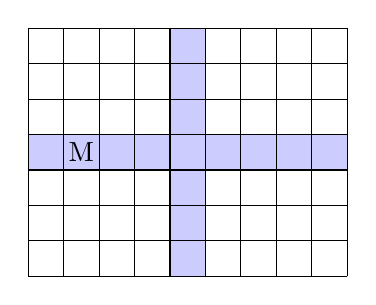
\begin{tikzpicture}[scale=0.45]
      % Grid dimensions
      \def\rows{7}
      \def\cols{9}

      % Draw grid
      \draw (0,0) grid (\cols,\rows);

      % Shade the center row (row 3)
      \foreach \x in {0,...,8} {
        \fill[blue!20] (\x,3) rectangle ++(1,1); % row 3 (y=2 to y=3)
      }

      % Shade the center column (column 4)
      \foreach \y in {0,...,6} {
        \fill[blue!20] (4,\y) rectangle ++(1,1); % column 4 (x=3 to x=4)
      }

      % Redraw grid lines on top
      \draw (0,0) grid (\cols,\rows);

      % Add text to a cell, e.g. row 5, col 2
      \node at (1.5,3.5) {M};
    \end{tikzpicture}
  \end{center}
  But is this algorithm correct? 
\end{frame}
\begin{frame}{Q3-5}
  There is a counterexample (see the picture in the same repository). 
\end{frame}
\iffalse
\begin{frame}{Q3-5}
  Now we prove that the given algorithm will always find a peak. Let $L_m$ (resp. $R_m$) denote the left (resp. right) half of $A$ without $C_m$. Let $M$ be the maximal element of $C_m$. 
  At each step, there are two possibilities:
  \begin{enumerate}
    \item $M$ is a (special) peak. Then we are done. 
    \item there is some $x > M$ in $L_m$ or $R_m$. Hence $x$ is strictly greater than all elements in the boundary $C_m$. 
  \end{enumerate}
  The correctness follows because if we keep falling into case 2., eventually we will be reduced to the case of only one column within our boundaries, in which case $M$ must be a peak by the condition in case 2.
  %\par It suffices to show that if $C_m$ does not contain a (special) peak, then there is a peak in $L_m$ or $R_m$. This is because if we keep getting non-peak column maximal, eventually we will be reduced to the case of a single column within our boundaries, in which case the column maximal will be peak within our boundaries. 
  %\par Let $M \in C_m$ be the maximal element of $C_m$. Then for it not to be peak, we must have some $x > M$ in $L_m$ or $R_m$. WLOG suppose $x \in$ $R_m$. Then we observe that the maximal element of $R_m$ will be a peak because it is greater than all elements on the boundary $C_m$. 
  \par In fact, this shows that we can focus our attention on just one of $L_m$ or $R_m$ (similar to binary search). 
\end{frame}
\begin{frame}{Q3-5}
  Hence we can actually have $T(n) = T(n/2)+c$ for number of columns. This gives $T(n) \in \Theta(\log{n})$ and hence overall complexity of $\Theta(m\log{n})$ if we do a clever modification. 
  \par Observe that there is an assymmetry between $m$ and $n$. If $m \approx n$, is there a faster way? Yes!
  \begin{center}
    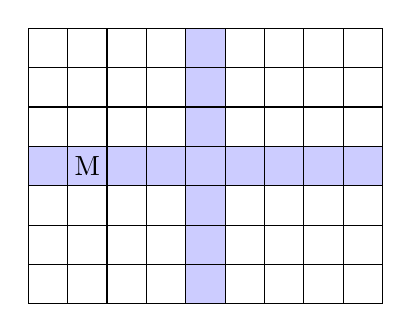
\begin{tikzpicture}[scale=0.5]
      % Grid dimensions
      \def\rows{7}
      \def\cols{9}

      % Draw grid
      \draw (0,0) grid (\cols,\rows);

      % Shade the center row (row 3)
      \foreach \x in {0,...,8} {
        \fill[blue!20] (\x,3) rectangle ++(1,1); % row 3 (y=2 to y=3)
      }

      % Shade the center column (column 4)
      \foreach \y in {0,...,6} {
        \fill[blue!20] (4,\y) rectangle ++(1,1); % column 4 (x=3 to x=4)
      }

      % Redraw grid lines on top
      \draw (0,0) grid (\cols,\rows);

      % Add text to a cell, e.g. row 5, col 2
      \node at (1.5,3.5) {M};
    \end{tikzpicture}
  \end{center}
  \par Now, add analogously a middle row $R_m$. We then compute the maximum $M$ over $R_m \cup C_m$ and recurse into one of the (up to) four smaller regions where $x>M$ lies. 
\end{frame}
\begin{frame}{Q3-5}
  Almost the same reasoning shows that this algorithm works. 
  \par Time complexity: wlog suppose $m \ge n$; let the running time be $F(m, n)$. Then we have
  \[F(m, n) = F(m/2, n/2)+cm, \]
  Hence
  \begin{align*}
    F(m, n) &= cm+cm/2+cm/4+\dots +c  \\ &\le cm(1+1/2+1/4+\dots) \in \Theta(m).
  \end{align*}
  \par Reference: the two pdfs from MIT which I have uploaded in our GitHub repository. 
\end{frame}
array([[ 1,  2, 99, 98, 22, 21, 20],
       [ 2,  3,  4,  6,  7,  8, 19],
       [ 3,  5,  6,  7,  8,  9, 18],
       [ 4,  6,  7,  8,  9, 10, 17],
       [ 6,  7,  8,  9, 10, 11, 16],
       [ 7,  8,  9, 10, 11, 12, 15],
       [ 8,  9, 10, 11, 12, 13, 14]])
\fi
\end{document}
